\documentclass{article}

% if you need to pass options to natbib, use, e.g.:
%     \PassOptionsToPackage{numbers, compress}{natbib}
% before loading neurips_2025

% ready for submission
% \usepackage{neurips_2025}

% to compile a preprint version, e.g., for submission to arXiv, add add the
% [preprint] option:
\usepackage[preprint]{neurips_2025}

% to compile a camera-ready version, add the [final] option, e.g.:
%     \usepackage[final]{neurips_2025}

% to avoid loading the natbib package, add option nonatbib:
%    \usepackage[nonatbib]{neurips_2025}

\usepackage[utf8]{inputenc} % allow utf-8 input
\usepackage[T1]{fontenc}    % use 8-bit T1 fonts
\usepackage{hyperref}       % hyperlinks
\usepackage{url}            % simple URL typesetting
\usepackage{booktabs}       % professional-quality tables
\usepackage{amsfonts}       % blackboard math symbols
\usepackage{nicefrac}       % compact symbols for 1/2, etc.
\usepackage{microtype}      % microtypography
\usepackage{xcolor}         % colors
\usepackage{natbib}
\usepackage{amsmath}
\usepackage{algorithm}
\usepackage{algorithmic}
\usepackage{graphicx}
\usepackage{subcaption}
\usepackage{multirow}
\usepackage{booktabs}
\usepackage{threeparttable}
\usepackage{adjustbox}

\bibliographystyle{unsrtnat} % Ensures bibliography style is set

\title{CRACK: Contrastive Relational-Aware Compression of Knowledge for Machine Learning Force Fields}

\author{
  Hyukjun Lim, Seokhyun Choung, Jeong Woo Han\thanks{Corresponding Author.} \\
  Department of Materials Science and Engineering \\
  Seoul National University \\
  \texttt{\{hyukjunlim, schoung9967, jwhan98\}@snu.ac.kr} \\
}

\begin{document}

\newcommand{\Lcrack}{\mathcal{L}_{\text{CRACK}}}
\newcommand{\Ltcr}{\mathcal{L}_{\text{TCR}}} % Teacher Contrastive Relational
\newcommand{\Lscr}{\mathcal{L}_{\text{SCR}}} % Student Contrastive Relational
\newcommand{\Ltask}{\mathcal{L}_{\text{task}}}
\newcommand{\Lnnton}{\mathcal{L}_{\text{n2n}}}
\newcommand{\Ltotal}{\mathcal{L}_{\text{total}}}

\maketitle

%%%%%%%%%%%%%%%%%%%%%%%%%%%%%%%%%%%%%%%%%%%%%%%%%%%%%%%%%%%%
\begin{abstract}
State-of-the-art equivariant Graph Neural Networks (GNNs) have significantly advanced molecular simulation by approaching quantum mechanical accuracy in predicting energies and forces. 
However, their substantial computational cost limits adoption in large-scale molecular dynamics simulations. 
Knowledge distillation (KD) offers a promising solution, but existing methods for Machine Learning Force Fields (MLFFs) often resort to simplistic atom-wise feature matching or complex second-order information distillation, overlooking fundamental first-order relational knowledge: how the teacher represents the potential energy surface (PES) through learned interatomic interactions. 
This paper introduces CRACK, \textbf{C}ontrastive \textbf{R}elational-\textbf{A}ware \textbf{C}ompression of \textbf{K}nowledge, a novel KD framework that directly distills interatomic relational knowledge by modeling each interaction as a \emph{relational vector} derived from bonded atom embeddings. 
CRACK employs contrastive learning to train students to generate relational vectors uniquely identifiable with teacher counterparts, effectively teaching the geometry of the teacher's learned PES.
On the challenging OC20 benchmark, CRACK enables a compact 22M-parameter student model to achieve superior energy and force prediction accuracy, significantly outperforming strong distillation baselines and demonstrating more effective transfer of physical knowledge.
\end{abstract}    


%%%%%%%%%%%%%%%%%%%%%%%%%%%%%%%%%%%%%%%%%%%%%%%%%%%%%%%%%%%%
\section{Introduction}

Graph Neural Networks (GNNs) have emerged as a dominant paradigm for machine learning on graph-structured data, demonstrating exceptional performance in a multitude of applications such as chemical reaction prediction, disease classification, recommendation systems, and social network analysis~\citep{zhou2020graph, gilmer2017neural, yang2023geometric, lim2025cheapnet}.
Their fundamental strength lies in their ability to iteratively aggregate information from node neighborhoods, thereby capturing the topological structure and feature information inherent in graphs~\citep{wu2020comprehensive, corso2024graph}.

Among the most impactful applications of GNNs is in computational chemistry and materials science, where the advent of Machine Learning Force Fields (MLFFs) has marked a paradigm shift in computational science. MLFFs enable the acceleration of discovery by providing tools that can approximate the accuracy of expensive quantum mechanical methods like Density Functional Theory (DFT) at a fraction of the computational cost~\citep{behler2007generalized, schutt2017schnet, unke2021machine}. 
Flagship equivariant Graph Neural Networks (GNNs), such as EquiformerV2~\citep{liao2023equiformerv2}, exemplify this progress, achieving state-of-the-art accuracy in predicting molecular energies and interatomic forces.

Despite their success, a central conflict persists: the trade-off between accuracy and computational efficiency.
The high fidelity of models like EquiformerV2 is often coupled with substantial computational demands, stemming from large parameter counts and complex operations such as higher-degree tensor products essential for capturing detailed geometric information.
This computational bottleneck restricts their routine application in critical research areas that necessitate simulations of large systems or over extended timescales, including high-throughput materials screening, the study of complex biomolecular dynamics, and various stages of drug discovery~\citep{unke2021machine}.

\begin{figure}[!tb]
    \centering
    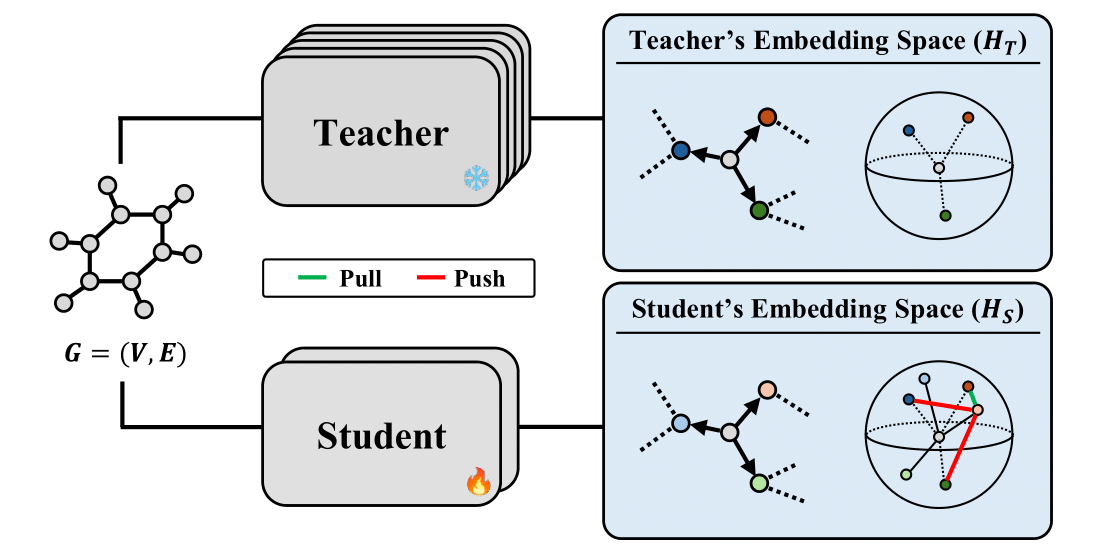
\includegraphics[width=0.9\textwidth]{CRACK_Overview.pdf}
    \caption{Overall Architecture of CRACK.} \label{fig.CRACK_Overview}
\end{figure}

Knowledge Distillation (KD) emerges as a key enabling technology to address this accuracy-efficiency dilemma~\citep{hinton2015distilling, gou2021knowledge}. 
The core principle of KD involves transferring the knowledge from a large, accurate \emph{teacher} MLFF to a smaller, computationally cheaper \emph{student} MLFF, with the goal of preserving the teacher's predictive performance in the compressed model.

However, the standard KD paradigm, often involving the minimization of Mean Squared Error (MSE) between teacher and student atom-wise hidden representations, can be fundamentally misaligned with the underlying physics when applied to MLFFs.
Such an approach treats atoms as independent data points, neglecting the fact that the crucial physical quantities—potential energy and interatomic forces—arise from the relative arrangements and interactions of atoms. 
The objective of an MLFF is not merely to replicate atomic feature vectors in isolation, but to accurately model the potential energy surface (PES) that these atoms collectively define through their interactions. 
The PES is inherently shaped by interatomic potentials, and while atomic embeddings encode environmental information, matching them directly does not guarantee that the nuanced representation of interactions, which dictates energy changes upon atomic displacement (i.e., forces), is faithfully transferred.

This paper advances the thesis, `\emph{To effectively distill an MLFF, one must distill the learned physics of interatomic potentials}'. 
Instead of asking `\emph{What are the features of this atom?}', we must ask the more fundamental question: `\emph{How does this atom interact with its neighbors?}'.

CRACK, \textbf{C}ontrastive \textbf{R}elational-\textbf{A}ware \textbf{C}ompression of \textbf{K}nowledge, is introduced as the first KD framework designed to directly and explicitly address this question for MLFFs. 
CRACK is built upon two conceptual pillars:
\begin{enumerate}
\item \textbf{Relational Vectors:} These are derived from the learned atomic embeddings (e.g., $z_{src} - z_{dst}$) and serve as proxies for the teacher's learned representation of the potential along a specific interatomic interaction.
\item \textbf{Contrastive Objective:} An InfoNCE-style loss~\citep{oord2018representation} is employed to train the student. This objective requires the student to produce relational vectors that are discriminatively similar to the teacher's corresponding relational vectors, effectively teaching the student the geometry of these interactions. This moves beyond simple regression of vector components to a more nuanced task of identifying and distinguishing specific interaction signatures learned by the teacher.
\end{enumerate}

The contributions of this work are summarized as follows:
\begin{itemize}
\item A novel, physics-informed knowledge distillation framework (CRACK) for MLFFs that, for the first time, directly distills first-order interatomic relational knowledge.
\item The formulation of a relational-contrastive loss function that explicitly aims to capture the geometry of the teacher model's learned potential energy surface, as manifested in pairwise atomic interactions.
\item Comprehensive empirical validation on the large-scale and challenging OC20 dataset~\citep{chanussot2021open}, demonstrating CRACK's state-of-the-art performance in compressing a powerful equivariant GNN (EquiformerV2) into a significantly smaller student model.
\end{itemize}


%%%%%%%%%%%%%%%%%%%%%%%%%%%%%%%%%%%%%%%%%%%%%%%%%%%%%%%%%%%%
\section{Related Work}

Knowledge distillation has become an increasingly explored avenue for compressing and enhancing GNNs. This section reviews prior work relevant to distilling knowledge in molecular GNNs and MLFFs, contextualizing the novel contributions of CRACK.


%%%%%%%%%%%%%%%%%%%%%%%%%%%%%%%%%%%%%%%%%%%%%%%%%%%%%%%%%%%%
\subsection{Knowledge Distillation for Molecular GNNs}

The application of knowledge distillation to molecular GNNs has shown promise for accelerating these computationally intensive models. 
\citet{ekstrom2023accelerating} established foundational evidence that KD is a viable strategy for improving the accuracy of student models in predicting molecular energies and forces. 
Their work focused on distilling hidden representations in directional and equivariant GNNs for regression tasks, demonstrating the general applicability of KD in this domain and providing empirical validation for the approach.


%%%%%%%%%%%%%%%%%%%%%%%%%%%%%%%%%%%%%%%%%%%%%%%%%%%%%%%%%%%%
\subsection{Feature-Based Distillation (Node-to-Node)}

The most prevalent approach for KD in molecular GNNs is feature-based distillation, as explored by \citet{ekstrom2023accelerating}. This method typically involves minimizing a regression loss, e.g., L1 or L2 norm, between the atom-wise embeddings or hidden states produced by the student and teacher models (referred to as n2n in this work). 
While computationally simple and often effective as a baseline, this approach is fundamentally limited from a physics perspective. 
As discussed in the Introduction, it treats atomic representations as independent entities, largely overlooking the relational nature of physical interactions that govern energies and forces in molecular systems.


%%%%%%%%%%%%%%%%%%%%%%%%%%%%%%%%%%%%%%%%%%%%%%%%%%%%%%%%%%%%
\subsection{Relational Knowledge Distillation (RKD)}

Moving beyond individual feature matching, \citet{park2019relational} introduced the concept of distilling relationships rather than isolated features in their seminal work on Relational Knowledge Distillation (RKD). 
Traditional RKD methods compute relations between all pairs of samples within a batch or all pairs of features within an instance. 
While innovative in principle, directly applying this framework to molecular graphs presents significant challenges. 
When "samples" are atoms, this approach can lead to physically meaningless comparisons, such as between arbitrary, non-bonded atoms across different molecules in a batch, and scales quadratically with the number of entities, making it computationally prohibitive for large molecular systems.

CRACK builds upon the conceptual foundation of RKD but instantiates it in a physically-grounded and graph-aware manner. In CRACK, relational vectors are defined specifically along physically meaningful interactions, which are the bonds identified by edges in the molecular graph. 
This restriction to O(E) relations, where E is the number of edges, makes CRACK both more physically relevant—distilling representations of actual interatomic potentials—and computationally scalable for large molecular systems.


%%%%%%%%%%%%%%%%%%%%%%%%%%%%%%%%%%%%%%%%%%%%%%%%%%%%%%%%%%%%
\subsection{Hessian-based Distillation}

Recently, more sophisticated KD methods have emerged that target higher-order physical information. 
\citet{amin2025towards} proposed distilling knowledge by matching the Hessians of energy predictions between a teacher foundation model and a smaller student MLFF. 
This approach captures the curvature of the potential energy surface (PES), which is crucial for understanding vibrational properties and reaction dynamics. 
While powerful in capturing second-order physical information, distilling Hessians involves computationally intensive second-order derivatives that may not always be available or stable, and may not be the most direct route to capturing fundamental interaction patterns.

CRACK differentiates itself by focusing on first-order relational information, specifically targeting the relational structure of the embedding space that defines pairwise potentials. 
This approach is arguably more direct in capturing the primary interactions that form the PES and may be more broadly applicable when Hessian information is noisy, unavailable, or computationally prohibitive. 
CRACK distills the geometry of learned pairwise potentials, representing a distinct yet equally fundamental aspect of the teacher's knowledge compared to PES curvature.


%%%%%%%%%%%%%%%%%%%%%%%%%%%%%%%%%%%%%%%%%%%%%%%%%%%%%%%%%%%%
\subsection{Contrastive Learning on Graphs}

Contrastive learning has emerged as a powerful paradigm for self-supervised representation learning on graphs, with methods like GRACE~\citep{zhu2020deep} and Deep Graph Infomax (DGI)~\citep{velivckovic2018deep} achieving notable success. 
These methods typically generate positive pairs through data augmentations such as two augmented views of the same node or graph and learn representations by contrasting positive pairs against negative pairs such as other nodes/graphs in the batch.

CRACK adopts a contrastive learning framework but operates within a fundamentally different paradigm: supervised distillation rather than self-supervised learning. Unlike conventional self-supervised contrastive methods that rely on data augmentation, CRACK leverages the teacher model as an explicit supervisory signal with two key distinctions:
\begin{itemize}
\item \textbf{Direct teacher-student correspondence:} Positive pairs are not generated through data augmentation but are explicitly defined by the correspondence between teacher and student representations of the \textit{same} interatomic interaction. For each interaction $k$, the teacher's relational vector $\mathbf{r}_{T,k}$ forms a positive pair with the student's corresponding relational vector $\mathbf{r}_{S,k}$.
\item \textbf{Physics-informed supervision:} This approach provides a stronger, more direct, and physically meaningful supervisory signal compared to augmentation-based methods. Rather than learning general invariance to augmentations, the student is explicitly guided to learn specific teacher-defined relational patterns that encode the physics of interatomic interactions.
\end{itemize}

This unique combination of relational distillation principles with a supervised contrastive objective, specifically tailored for the physics of MLFFs, enables CRACK to occupy a distinct methodological niche in the knowledge distillation landscape. 
Unlike generic RKD approaches that may include physically meaningless relations or self-supervised contrastive methods that rely on data augmentation, CRACK is designed to directly and selectively transfer the teacher's learned representation of specific interatomic interactions. 
This targeted approach, guided by explicit teacher supervision for each molecular interaction, facilitates more faithful and physically meaningful transfer of the teacher's learned potential energy surface geometry.


%%%%%%%%%%%%%%%%%%%%%%%%%%%%%%%%%%%%%%%%%%%%%%%%%%%%%%%%%%%%
\section{Methods}

This section details the CRACK framework, beginning with preliminary definitions, followed by the formulation of relational vectors and the contrastive distillation objective.


%%%%%%%%%%%%%%%%%%%%%%%%%%%%%%%%%%%%%%%%%%%%%%%%%%%%%%%%%%%%
\subsection{Preliminaries}

A molecule is represented as a graph $\mathcal{G} = (\mathcal{V}, \mathcal{E})$, where $\mathcal{V}$ is the set of $N$ atoms (nodes) and $\mathcal{E}$ is the set of $E$ interatomic interactions (edges). Each atom $i \in \mathcal{V}$ is associated with initial features $\mathbf{h}_i^{(0)}$.

The \textbf{teacher model}, denoted $f_T$ with parameters $\theta_T$, is a pre-trained, large-capacity equivariant GNN. It outputs final node embeddings $\mathbf{Z}_T = \{\mathbf{z}_{T,1}, \dots, \mathbf{z}_{T,N}\}$, where $\mathbf{z}_{T,i} \in \mathbb{R}^{D_T}$. 
The \textbf{student model}, $f_S$ with parameters $\theta_S$, is a smaller GNN. It produces node embeddings $\mathbf{Z}_S' \in \mathbb{R}^{N \times D_S}$. A linear projection head $P: \mathbb{R}^{D_S} \to \mathbb{R}^{D_T}$ maps the student's embeddings to the teacher's dimension, yielding $\mathbf{Z}_S = P(\mathbf{Z}_S')$.

The primary task of an MLFF is to predict the total potential energy $U$ and per-atom forces $\mathbf{F}_i$.


%%%%%%%%%%%%%%%%%%%%%%%%%%%%%%%%%%%%%%%%%%%%%%%%%%%%%%%%%%%%
\subsection{CRACK: Distilling the Geometry of Interatomic Potentials}

The core intuition is that the directional vector difference $\mathbf{z}_{T,i} - \mathbf{z}_{T,j}$ for a bonded pair $(i, j)$ serves as a learned proxy for the interaction potential. CRACK aims to teach the student to replicate the \textit{geometry} of this relational space.

%%%%%%%%%%%%%%%%%%%%%%%%%%%%%%%%%%%%%%%%%%%%%%%%%%%%%%%%%%%%
\subsubsection{Formalizing Relational Vectors}

For each edge $e_k = (i,j) \in \mathcal{E}$, we define teacher and student relational vectors, $\mathbf{r}_{T,k}$ and $\mathbf{r}_{S,k}$. Let $\mathbf{z}_{T,i}$ and $\mathbf{z}_{S,i}$ denote the embeddings of atom $i$ in the teacher and student models, respectively.

First, the atom embeddings are L2 normalized:
$$ \hat{\mathbf{z}}_{T,i} = \frac{\mathbf{z}_{T,i}}{\|\mathbf{z}_{T,i}\|_2}, \quad \hat{\mathbf{z}}_{S,i} = \frac{\mathbf{z}_{S,i}}{\|\mathbf{z}_{S,i}\|_2} $$
Next, for an edge $e_k = (\text{src}, \text{dst})$, the raw difference vectors are computed:
$$ \mathbf{x}_{T,k} = \hat{\mathbf{z}}_{T,\text{src}} - \hat{\mathbf{z}}_{T,\text{dst}}, \quad \mathbf{x}_{S,k} = \hat{\mathbf{z}}_{S,\text{src}} - \hat{\mathbf{z}}_{S,\text{dst}} $$
Finally, these difference vectors are themselves L2 normalized to yield the relational vectors, which focuses the loss on their direction:
$$ \mathbf{r}_{T,k} = \frac{\mathbf{x}_{T,k}}{\|\mathbf{x}_{T,k}\|_2}, \quad \mathbf{r}_{S,k} = \frac{\mathbf{x}_{S,k}}{\|\mathbf{x}_{S,k}\|_2} $$


%%%%%%%%%%%%%%%%%%%%%%%%%%%%%%%%%%%%%%%%%%%%%%%%%%%%%%%%%%%%
\subsubsection{The Contrastive Objective}

CRACK employs an InfoNCE-based loss~\citep{oord2018representation}. For a batch of $E_b$ interactions, the student's relational vector $\mathbf{r}_{S,k}$ is the positive sample for the teacher's $\mathbf{r}_{T,k}$. All other student vectors $\mathbf{r}_{S,m}$ where $m \neq k$ are negative samples.

The CRACK loss function is formally defined as:
$$ \Lcrack = - \frac{1}{E_b} \sum_{k=1}^{E_b} \log \frac{\exp(\text{sim}(\mathbf{r}_{T,k}, \mathbf{r}_{S,k}) / \tau)}{\sum_{m=1}^{E_b} \exp(\text{sim}(\mathbf{r}_{T,k}, \mathbf{r}_{S,m}) / \tau)} $$
where $\text{sim}(\mathbf{u}, \mathbf{v}) = \mathbf{u}^\top \mathbf{v}$ is the cosine similarity since vectors are normalized, and $\tau$ is a temperature hyperparameter. This is equivalent to a cross-entropy loss over the similarity logits, where the target for each teacher vector $\mathbf{r}_{T,k}$ is its corresponding student vector $\mathbf{r}_{S,k}$.


%%%%%%%%%%%%%%%%%%%%%%%%%%%%%%%%%%%%%%%%%%%%%%%%%%%%%%%%%%%%
\subsection{Overall Training Objective}

The student model is trained by minimizing a composite loss:
$$ \Ltotal = \Ltask + \lambda_1 \Lcrack + \lambda_2 L_{\text{KD}} $$
where $\Ltask$ is the standard energy/force prediction loss, $L_{\text{KD}}$ is the optional knowledge distillation loss, such as node-to-node feature matching loss ($\sum_i ||\mathbf{z}_{S,i} - \mathbf{z}_{T,i}||^2_2$), and $\lambda_1, \lambda_2$ are balancing hyperparameters.


%%%%%%%%%%%%%%%%%%%%%%%%%%%%%%%%%%%%%%%%%%%%%%%%%%%%%%%%%%%%
\section{Experiments}
This section details the experimental setup, presents main results, and includes ablation studies.
Further experimental details and code are available at \href{https://github.com/hyukjunlim/CRACK}{https://github.com/hyukjunlim/CRACK}.


%%%%%%%%%%%%%%%%%%%%%%%%%%%%%%%%%%%%%%%%%%%%%%%%%%%%%%%%%%%%
\subsection{Experimental Setup}
\textbf{Dataset:} Open Catalyst 2020 (OC20)~\citep{chanussot2021open}, using the O* and 200K subsets.

\textbf{Models:} Teacher model is 153M-parameter EquiformerV2~\citep{liao2023equiformerv2} with 20 message passing layers. Student model is 22M-parameter EquiformerV2 with only 2 message passing layers, same architecture as teacher but with reduced depth. 
Since the architectures are identical, we can initialize the student by loading the first two message passing layers from the pretrained teacher model (denoted as "pretrained" baseline).

\textbf{Evaluation Protocol:} We report Energy MAE (meV) and Force MAE (meV/Å). Optionally, we also report the MAE and Cosine Similarity of the final layer embeddings of the student compared to the teacher.

\textbf{Baselines:} Teacher models, Student trained from scratch (vanilla), Student initialized with first two layers of teacher (pretrained), direct feature distillation (n2n)~\citep{ekstrom2023accelerating}, and Hessian-based distillation~\citep{amin2025towards}.


%%%%%%%%%%%%%%%%%%%%%%%%%%%%%%%%%%%%%%%%%%%%%%%%%%%%%%%%%%%%
\subsection{Main Results}

\textbf{Analysis of O* Subset:} As shown in Table \ref{tab:crack-oc20}, our CRACK method with n2n achieves the best energy MAE (232.0 meV) and force MAE (5.8 meV/Å) among student models. 
This is a substantial improvement over the strong n2n baseline, demonstrating the clear benefit of adding relational distillation.

\begin{table}[htbp]
\centering
\caption{Performance of CRACK on O* subset of OC20 dataset. The best results are highlighted in \textbf{bold}. Second best results are \underline{underlined}.}
\label{tab:crack-oc20}
\begin{adjustbox}{max width=0.8\textwidth}
\begin{threeparttable}
\begin{tabular}{cccccc}
\toprule
\multirow{2}{*}{\textbf{Method}} & \multirow{2}{*}{\textbf{Params}} & \multicolumn{2}{c}{\textbf{Embedding}} & \textbf{Energy} & \textbf{Force} \\
\cmidrule(lr){3-6}
 & & MAE & Cosine Similarity & MAE (meV) $\downarrow$ & MAE (m eV/Å) $\downarrow$ \\
\midrule
Teacher$^*$ & 153M & - & - & 39.8 & 5.8 \\
Teacher & 83M & - & - & 110.7 & 6.9 \\
Teacher & 31M & - & - & 54.1 & 6.1 \\
\midrule
vanilla & 22M & 0.217 & 0.205 & 294.5 & 5.9 \\ 
pretrained & 22M & 0.311 & 0.271 & 263.6 & 6.1 \\ 
n2n & 22M & 0.078 & 0.839 & 252.9 & \textbf{5.8} \\ 
Hessian & 22M & 1.062 & 0.073 & 363.5 & 26.1 \\ 
\midrule
% Ours (instance-level) & 22M & 0.258 & 0.210 & 241.5 & 6.1 \\ 
% Ours (instance-level, w/ n2n) & 22M & 0.081 & 0.828 & 235.7 & \textbf{5.8} \\ 
Ours & 22M & 0.282 & 0.230 & \underline{234.1} & 6.1 \\ 
Ours (w/ n2n) & 22M & 0.082 & 0.820 & \textbf{231.7} & \textbf{5.8} \\ 
\bottomrule 
\end{tabular}
\begin{tablenotes}
\small
\item[*] The teacher model used for knowledge distillation. Loaded from EquiformerV2.
\end{tablenotes}
\end{threeparttable}
\end{adjustbox}
\end{table}

\textbf{Analysis of 200K Subset:} This trend is confirmed on the 200K subset (Table \ref{tab:crack-oc20-200k}). CRACK alone achieves the best energy MAE, while the combined method excels in force MAE. 
This suggests CRACK is particularly effective at capturing the global energy landscape, while n2n helps ground local features crucial for forces.

\begin{table}[htbp]
\centering
\caption{Performance of CRACK on 200K subset of OC20 dataset. The best results are highlighted in \textbf{bold}. Second best results are \underline{underlined}.}
\label{tab:crack-oc20-200k}
\begin{adjustbox}{max width=0.8\textwidth}
\begin{threeparttable}
\begin{tabular}{cccccc}
\toprule
\multirow{2}{*}{\textbf{Method}} & \multirow{2}{*}{\textbf{Params}} & \multicolumn{2}{c}{\textbf{Embedding}} & \textbf{Energy} & \textbf{Force} \\
\cmidrule(lr){3-6}
 & & MAE & Cosine Similarity & MAE (meV) $\downarrow$ & MAE (meV/Å) $\downarrow$ \\
\midrule
Teacher$^*$ & 153M & - & - & 171.5 & 12.4 \\
Teacher & 83M & - & - & 221.0 & 16.5 \\
Teacher & 31M & - & - & 177.5 & 14.0 \\
\midrule
vanilla & 22M & 0.309 & 0.233 & 474.9 & 51.8 \\ 
pretrained & 22M & 0.181 & 0.460 & 410.8 & 37.6 \\ 
n2n & 22M & 0.096 & 0.816 & 412.8 & \underline{34.8} \\ 
Hessian & 22M & 0.351 & 0.180 & 419.3 & 48.6 \\ 
\midrule
% Ours (instance-level) & 22M & 0.187 & 0.410 & 373.7 & 36.2 \\ 
% Ours (instance-level, w/ n2n) & 22M & 0.097 & 0.813 & 380.6 & 34.2 \\ 
Ours & 22M & 0.190 & 0.424 & \underline{373.8} & 35.8 \\ 
Ours (w/ n2n) & 22M & 0.097 & 0.811 & \textbf{371.1} & \textbf{34.1} \\ 
\bottomrule 
\end{tabular}
\begin{tablenotes}
\small
\item[*] The teacher model used for knowledge distillation. Loaded from EquiformerV2.
\end{tablenotes}
\end{threeparttable}
\end{adjustbox}
\end{table}


%%%%%%%%%%%%%%%%%%%%%%%%%%%%%%%%%%%%%%%%%%%%%%%%%%%%%%%%%%%%
\subsection{Ablation Studies}
\subsubsection{Relational vs. Instance-Level Contrastive Loss} 
The performance of instance-level contrastive loss applied directly to atom embeddings $(\mathbf{z}_{S,i}, \mathbf{z}_{T,i})$ was compared to CRACK's relational approach. 
Table \ref{tab:crack-instance-relational} shows the results of the experiment conducted on the O* subset of OC20 dataset.
The consistent superiority of the relational method, especially in energy MAE, validates our central hypothesis: distilling interactions is more effective than distilling isolated atom features.

\begin{table}[htbp]
\centering
\caption{Performance of instance-level contrastive loss compared to relational-level contrastive loss. The best results are highlighted in \textbf{bold}. Second best results are \underline{underlined}.}
\label{tab:crack-instance-relational}
\begin{adjustbox}{max width=0.8\textwidth}
\begin{threeparttable}
\begin{tabular}{cccccc}
\toprule
\multirow{2}{*}{\textbf{Method}} & \multirow{2}{*}{\textbf{Params}} & \multicolumn{2}{c}{\textbf{Embedding}} & \textbf{Energy} & \textbf{Force} \\
\cmidrule(lr){3-6}
& & MAE & Cosine Similarity & MAE (meV) $\downarrow$ & MAE (meV/Å) $\downarrow$ \\
\midrule
instance-level & 22M & 0.258 & 0.210 & 241.5 & 6.1 \\ 
instance-level, w/ n2n & 22M & 0.081 & 0.828 & 235.7 & \textbf{5.8} \\ 
relational-level & 22M & 0.282 & 0.230 & \underline{234.1} & 6.1 \\ 
relational-level, w/ n2n & 22M & 0.082 & 0.820 & \textbf{232.0} & \textbf{5.8} \\ 
\bottomrule 
\end{tabular}
\end{threeparttable}
\end{adjustbox}
\end{table}
        
\subsubsection{Impact of Temperature $\tau$} 
The temperature $\tau$ controls the difficulty of the contrastive task. 
A low $\tau$ increases discrimination but risks instability, while a high $\tau$ may wash out important details. 
An optimal $\tau=0.15$ was found empirically to balance these trade-offs.

\begin{table}[htbp]
\centering
\caption{Performance of CRACK with different temperature $\tau$. The best results are highlighted in \textbf{bold}. Second best results are \underline{underlined}.}
\label{tab:crack-temperature}
\begin{adjustbox}{max width=0.7\textwidth}
\begin{threeparttable}
\begin{tabular}{cccccc}
\toprule
\multirow{2}{*}{\textbf{$\tau$}} & \multirow{2}{*}{\textbf{Params}} & \multicolumn{2}{c}{\textbf{Embedding}} & \textbf{Energy} & \textbf{Force} \\

\cmidrule(lr){3-6}
& & MAE & Cosine Similarity & MAE (meV) $\downarrow$ & MAE (meV/Å) $\downarrow$ \\
\midrule
0.05 & 22M & 0.085 & 0.806 & 234.0 & 5.8 \\ 
0.07 & 22M & 0.084 & 0.810 & 232.9 & 5.8 \\ 
0.1 & 22M & 0.083 & 0.814 & 232.0 & 5.8 \\ 
0.15 & 22M & 0.082 & 0.820 & 232.0 & 5.8 \\ 
0.2 & 22M & 0.082 & 0.823 & 232.9 & 5.8 \\ 
\bottomrule 
\end{tabular}
\end{threeparttable}
\end{adjustbox}
\end{table}


%%%%%%%%%%%%%%%%%%%%%%%%%%%%%%%%%%%%%%%%%%%%%%%%%%%%%%%%%%%%
\section{Conclusion and Future Work}
\subsection{Summary of Findings}

This paper introduced CRACK, \textbf{C}ontrastive \textbf{R}elational-\textbf{A}ware \textbf{C}ompression of \textbf{K}nowledge, a novel knowledge distillation framework specifically designed for Machine Learning Force Fields (MLFFs). 
CRACK represents a fundamental shift in how we approach knowledge distillation for MLFFs by directly targeting the learned physics of interatomic potentials rather than treating atoms as independent entities.
This is achieved by defining relational vectors from the embeddings of bonded atoms and using contrastive learning to train students to generate relational vectors uniquely identifiable with teacher counterparts, effectively teaching the geometry of the teacher's learned potential energy surface.

Extensive experiments on the challenging OC20 dataset demonstrated that CRACK enables a compact 22M-parameter student model to significantly outperform strong distillation baselines, achieving superior energy and force prediction accuracy compared to conventional node-to-node feature matching approaches.
The ablation studies confirmed the critical contribution of the proposed relational contrastive distillation loss, validating our central hypothesis that distilling interactions is more effective than distilling isolated atomic features.


%%%%%%%%%%%%%%%%%%%%%%%%%%%%%%%%%%%%%%%%%%%%%%%%%%%%%%%%%%%%
\subsection{Limitations}

While CRACK shows promising results, certain limitations exist. 
The contrastive distillation process, which compares relational vectors within each batch, can be computationally intensive for very large molecular systems.
The current work exclusively defined relational vectors as the difference between bonded atom embeddings; more sophisticated relational definitions incorporating angular information or higher-order structural features might yield further improvements but could also increase complexity. 
Finally, the optimal balance between task loss, conventional knowledge distillation, and CRACK loss can be dataset-dependent, requiring careful hyperparameter tuning.


%%%%%%%%%%%%%%%%%%%%%%%%%%%%%%%%%%%%%%%%%%%%%%%%%%%%%%%%%%%%
\subsection{Future Directions}

One promising direction is exploring more sophisticated relational descriptors, moving beyond simple vector differences to incorporate angular relationships, three-body interactions, or attention-based scores that capture more nuanced aspects of the potential energy surface.
Improving the scalability of CRACK to massive molecular systems is also critical, which could be achieved by developing more efficient negative sampling strategies for the contrastive loss rather than using all in-batch relations.
Furthermore, combining CRACK's first-order distillation with second-order Hessian-based methods could capture a more complete spectrum of physical knowledge, potentially leading to even more faithful transfer of the teacher's understanding.
Finally, the core principles of CRACK could be generalized beyond MLFFs to other domains where relational knowledge is important, such as social network analysis, recommendation systems, or other molecular property prediction tasks, suggesting broader applicability of the relational-contrastive distillation concept.

In conclusion, CRACK offers a significant step towards more effective knowledge distillation for MLFFs by enabling the transfer of fundamental physical understanding through interatomic relationships, paving the way for more efficient yet accurate molecular simulations.


%%%%%%%%%%%%%%%%%%%%%%%%%%%%%%%%%%%%%%%%%%%%%%%%%%%%%%%%%%%%
% \begin{ack}
% Placeholders for acknowledgments.
% \end{ack}

%%%%%%%%%%%%%%%%%%%%%%%%%%%%%%%%%%%%%%%%%%%%%%%%%%%%%%%%%%%%
\bibliography{neurips_2025} % Ensure your .bib file is named neurips_2025.bib or adjust accordingly

%%%%%%%%%%%%%%%%%%%%%%%%%%%%%%%%%%%%%%%%%%%%%%%%%%%%%%%%%%%%
\appendix

\section{Experimental Details}
This section provides supplementary details regarding the experimental setup, including dataset statistics, implementation specifics, and model architectures.

\subsection{Dataset Statistics}
The Open Catalyst 2020 (OC20) dataset is a large-scale quantum mechanics dataset for catalysis. We use two of its sub-splits for our experiments: the O* subset and the 200K subset. The O* subset is a specialized, out-of-distribution set designed to test model generalization on unseen adsorbates. The 200K subset is a larger, more diverse training set. Key statistics for these subsets are provided in Table \ref{tab:dataset-stats}.

\begin{table}[h]
\centering
\caption{Statistics for the OC20 Subsets Used in This Work.}
\label{tab:dataset-stats}
\begin{adjustbox}{max width=0.8\textwidth}
\begin{tabular}{lcc}
\toprule
\textbf{Statistic} & \textbf{O* Subset} & \textbf{200K Subset} \\
\midrule
Total Number of Structures & 459,715 & 198,823 \\
Number of Adsorbates & 1 & 82 \\
Number of Catalyst Surfaces & 55 & 55 \\
Adsorbate Formula & O* & Various \\
\bottomrule
\end{tabular}
\end{adjustbox}
\end{table}

\subsection{Implementation Details}
All models were trained using the AdamW optimizer. The learning rate was warmed up to a peak value of $5 \times 10^{-4}$ over 30,000 steps and then decayed using a cosine schedule. The batch size was set to 4. The loss balancing hyperparameters were empirically set to $\lambda_1=10.0$ for the CRACK loss and $\lambda_2=1.0$ for the n2n feature matching loss. Based on our ablation studies, the temperature for the contrastive loss was set to $\tau=0.15$. All experiments were conducted on NVIDIA A6000 or A5000 GPUs, separately.

\begin{table}[h]
\centering
\caption{Key Hyperparameters for Training.}
\label{tab:hyperparams}
\begin{adjustbox}{max width=0.7\textwidth}
\begin{tabular}{lc}
\toprule
\textbf{Hyperparameter} & \textbf{Value} \\
\midrule
Optimizer & AdamW \\
Learning Rate Schedule & Cosine Decay w/ Warmup \\
Peak Learning Rate & $5 \times 10^{-4}$ \\
Warmup Steps & 30,000 \\
Batch Size & 4 \\
$\Lcrack$ weight ($\lambda_1$) & 10.0 \\
$L_{\text{KD}}$ weight ($\lambda_2$) & 1.0 \\
Temperature ($\tau$) & 0.15 \\
\bottomrule
\end{tabular}
\end{adjustbox}
\end{table}

% \subsection{Model Architectures}
% \textbf{Teacher Model:} The teacher is the 153M-parameter EquiformerV2 model. It consists of 20 message passing blocks, a feed-forward network dimension of 512, 8 attention heads, and uses degree 3 tensor products.

% \textbf{Student Model:} The student model is a significantly smaller 22M-parameter EquiformerV2. It shares the same architecture as the teacher but with its depth drastically reduced to only 2 message passing blocks. The embedding dimension for the student is 256, which is mapped to the teacher's dimension of 512 using a linear projection head during distillation.


%%%%%%%%%%%%%%%%%%%%%%%%%%%%%%%%%%%%%%%%%%%%%%%%%%%%%%%%%%%%
\section{Training Algorithm}
This section provides the detailed pseudocode for the end-to-end training procedure of CRACK, as described in the main paper.
\begin{algorithm}[H]
    \caption{Contrastive Relational-Aware Compression of Knowledge (CRACK) Training}
    \label{alg:crack}
    \begin{algorithmic}[1]
    \STATE \textbf{Input:} Training data loader $\mathcal{D}$, pre-trained teacher model $f_T$, student model $f_S$, projection head $P$.
    \STATE \textbf{Input:} Hyperparameters: learning rate $\eta$, loss weights $\lambda_1, \lambda_2$, temperature $\tau$.
    \STATE Initialize parameters $\theta_S$ of $f_S$ and $\theta_P$ of $P$.
    \STATE Freeze parameters of the teacher model $f_T$.
    \FOR{each training epoch}
        \FOR{each batch of molecular graphs $\{\mathcal{G}\}$ in $\mathcal{D}$}
            \STATE \textit{// Generate embeddings from teacher and student models}
            \STATE With no gradient tracking for $f_T$:
            \STATE $\mathbf{Z}_T \leftarrow f_T(\{\mathcal{G}\})$  \COMMENT{Teacher atom embeddings, size $N_{batch} \times D_T$}
            \STATE $\mathbf{Z}'_S \leftarrow f_S(\{\mathcal{G}\})$ \COMMENT{Student atom embeddings, size $N_{batch} \times D_S$}
            \STATE $\mathbf{Z}_S \leftarrow P(\mathbf{Z}'_S)$ \COMMENT{Projected student embeddings, size $N_{batch} \times D_T$}
            
            \STATE \textit{// Compute standard task loss (Energy and Forces)}
            \STATE $U_S, \mathbf{F}_S \leftarrow \text{Predictions from } f_S$
            \STATE $\Ltask \leftarrow \text{Loss}( (U_S, \mathbf{F}_S), (U_{true}, \mathbf{F}_{true}) )$
            
            \STATE \textit{// Compute optional node-to-node KD loss}
            \STATE $L_{\text{KD}} \leftarrow \frac{1}{N_{batch}} \sum_{i=1}^{N_{batch}} ||\mathbf{z}_{S,i} - \mathbf{z}_{T,i}||^2_2$

            \STATE \textit{// Construct Relational Vectors for all E edges in the batch}
            \STATE For each edge $e_k = (\text{src}, \text{dst})$:
            \STATE Normalize atom embeddings: $\hat{\mathbf{z}} = \mathbf{z} / ||\mathbf{z}||_2$
            \STATE Compute normalized difference vectors: $\mathbf{r}_k = (\hat{\mathbf{z}}_{\text{src}} - \hat{\mathbf{z}}_{\text{dst}}) / ||\hat{\mathbf{z}}_{\text{src}} - \hat{\mathbf{z}}_{\text{dst}}||_2$
            \STATE This yields teacher set $\{\mathbf{r}_{T,k}\}$ and student set $\{\mathbf{r}_{S,k}\}$.

            \STATE \textit{// Compute CRACK contrastive loss}
            \STATE $\Lcrack \leftarrow - \frac{1}{E_{batch}} \sum_{k=1}^{E_{batch}} \log \frac{\exp(\mathbf{r}_{T,k} \cdot \mathbf{r}_{S,k} / \tau)}{\sum_{m=1}^{E_{batch}} \exp(\mathbf{r}_{T,k} \cdot \mathbf{r}_{S,m} / \tau)}$
            
            \STATE \textit{// Compute total loss and update student model}
            \STATE $\Ltotal \leftarrow \Ltask + \lambda_1 \Lcrack + \lambda_2 L_{\text{KD}}$
            \STATE Update parameters $(\theta_S, \theta_P)$ using gradient descent on $\Ltotal$.
        \ENDFOR
    \ENDFOR
    \STATE \textbf{Output:} Trained student model $f_S$. The projection head $P$ is discarded after training.
    \end{algorithmic}
\end{algorithm}

%%%%%%%%%%%%%%%%%%%%%%%%%%%%%%%%%%%%%%%%%%%%%%%%%%%%%%%%%%%%
\end{document}
